\documentclass[11pt]{article}

\usepackage{times}
\usepackage{graphicx}
\usepackage{url}
\usepackage{hyperref}

\textwidth=6.5in
\textheight=8.75in
\oddsidemargin=0.0in
\evensidemargin=0.0in
\topmargin=-0.5in

\begin{document}
\thispagestyle{empty}

\begin{center}
{\bf CS 6300} \hfill {\large\bf HW02:  Minimax and Alpha-Beta Pruning} \hfill {\bf Due January 30, 2023}
\end{center}

Please use \LaTeX\ to produce your writeups. See the Homework Assignments 
page on the class website for details.

For these problems the easiest way to "write" your solutions is probably to download the file \texttt{gametree.png}, insert it into a google slide deck, then insert text to write your answers, export as a png and put that in your latex write up.


\section{Minimax}

For the following game tree, carry out minimax search. Give the value for each node.

\begin{center}
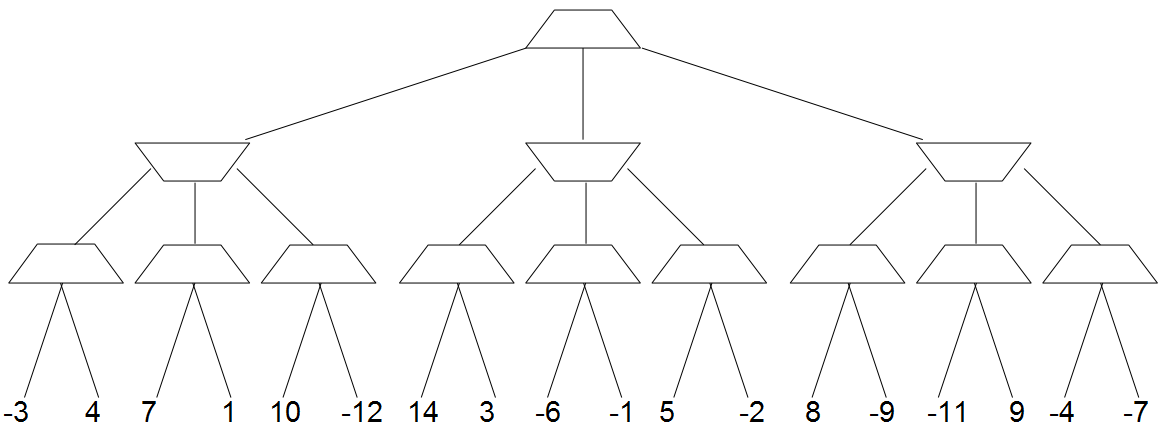
\includegraphics[width=\linewidth]{gametree.png}
\end{center}

\bf Solution:

\begin{center}
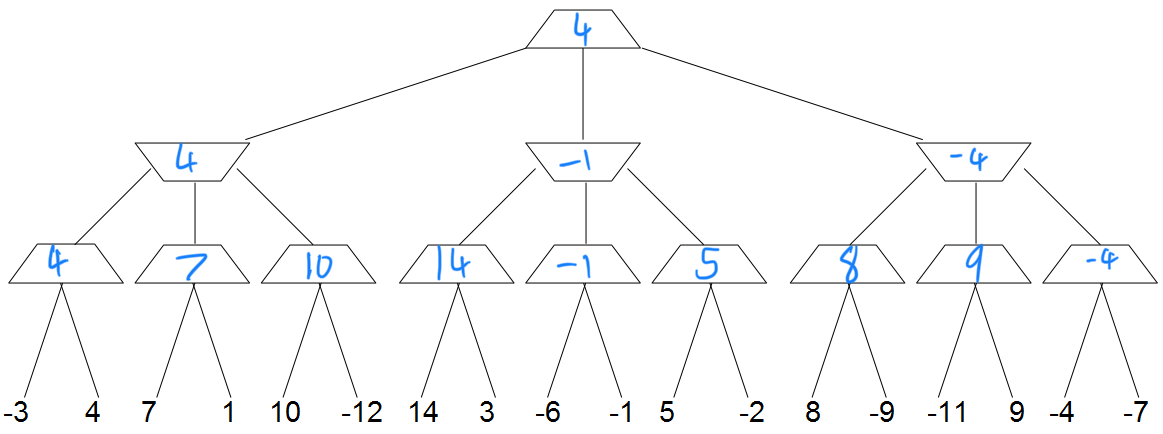
\includegraphics[width=\linewidth]{Q1.png}
\end{center}

\pagebreak

\section{Alpha-Beta pruning}
For the same game tree perform alpha-beta pruning. Let $(\alpha, \beta)_{i}$ be the
  $\alpha$-$\beta$ values passed down an edge to node $i$, etc., for all
  the nodes with appropriate change of index or indices.  Similarly,
  $v_i$ is the value passed up edge $i$, etc..  Show the sequence of
  steps, by giving the $(\alpha, \beta)$ values on the way down, and the $v$ values
  on the way up. See the example in the Practice Problems on the class website.
  \url{https://www.cs.utah.edu/~dsbrown/classes/cs6300/practice/minimax_practice_sol.pdf}
Cross out the branches
that are pruned.

\begin{center}
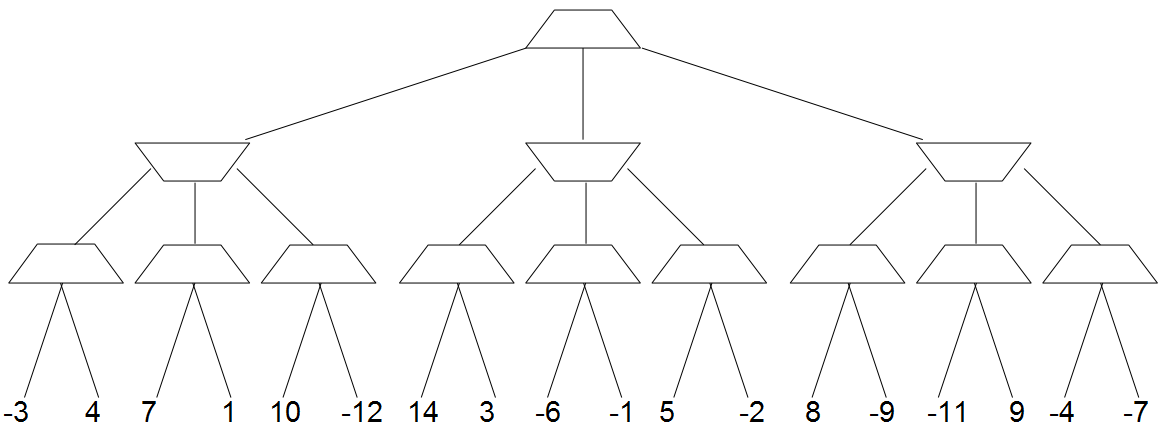
\includegraphics[width=\linewidth]{gametree.png}
\end{center}

\bf Solution:

\begin{center}
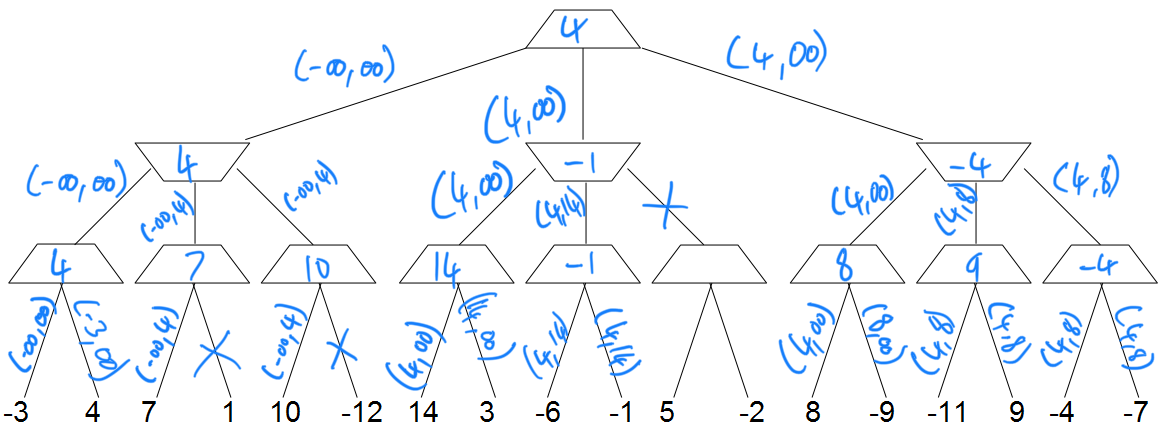
\includegraphics[width=\linewidth]{Q2.png}
\end{center}

\end{document}
